\documentclass[11pt]{article}

\usepackage[T1]{fontenc}
\usepackage{amsmath,amssymb,amsthm}
\usepackage{array}
\usepackage{booktabs}
\usepackage{geometry}
\usepackage{graphicx}
\usepackage{hyperref}
\usepackage{microtype}
\usepackage{placeins}
\usepackage{xcolor}
\usepackage{xurl}

\geometry{margin=0.9in}
\graphicspath{{./}}
\hypersetup{
  colorlinks=true,
  linkcolor=blue!55!black,
  citecolor=blue!55!black,
  urlcolor=blue!55!black
}

\newcommand{\CC}{\mathbb{C}}
\newcommand{\ee}{\mathrm{e}}
\newcommand{\ii}{\mathrm{i}}
\newcommand{\fro}{\mathrm{F}}
\newcommand{\mat}[1]{\mathsf{#1}}
\newcommand{\code}[1]{\texttt{#1}}
\newcommand{\eref}{E_{\mathrm{ref}}}
\newcolumntype{L}[1]{>{\raggedright\arraybackslash}p{#1}}
\newtheorem{proposition}{Proposition}
\newtheorem{corollary}{Corollary}

\title{Gauge Alignment and Block-Hopping Locality in a Controlled\\
Rank-Two Periodic One-Dimensional Composite Band}
\author{Eugene Joseph M. Ragasa\\
De La Salle University, Manila\\
\texttt{eugene.ragasa@dlsu.edu.ph}}
\date{Draft technical report --- \today}

\begin{document}
\maketitle

\begin{abstract}
A composite band is represented by a matrix-valued Hamiltonian whose real-space block
hoppings depend on the reciprocal-space frame chosen inside the retained subspace.  We
study that dependence in an exact four-state, one-dimensional periodic parent with a
rank-two retained spectral space.  A polar-transported reference frame is subjected to
a prescribed smooth right-unitary rotation, then compared with pointwise and
one-global-unitary Procrustes alignment.  Complete 64-point block Fourier transforms
and symmetric range truncations are assessed on both the construction mesh and an
exactly disjoint 257-point staggered mesh.  The sampled retained/excluded gap and
transport-overlap gates pass.  Pointwise alignment recovers reference frames and
represented operators at binary64 roundoff, whereas one global unitary does not.  The
reference and pointwise channels have rapidly decaying block hoppings and reach
roundoff-scale spectral truncation errors by range eight.  The attacked channel retains
an evaluation spectral error of approximately $7.04\times10^{-5}\eref$ at the same
range despite having the same exact pointwise spectra before truncation.  Cyclic
negative-Nyquist conversion power, complete-interpolant error, deliberate-truncation
error, and total consequence are reported separately in both normalized Hamiltonian and
sorted-band metrics.  An independent numerical route reconstructs every authoritative
value and the authenticated plotting projection; all 56 comparisons pass with maximum
discrepancy $1.42\times10^{-14}$.  These are provisional finite-control results.  They do not
establish continuum convergence, material validity, uncertainty quantification,
publication acceptance, release, or evidence sealing.
\end{abstract}

\noindent\textbf{Keywords:} composite band; gauge alignment; block hopping; Fourier
locality; Procrustes problem; independent verification

\section{Scientific question and evidence boundary}

For a fixed isolated rank-two spectral subspace of an exact finite periodic parent,
how do a declared reciprocal-space frame attack, pointwise right-unitary alignment,
and one-global-unitary alignment change represented Hamiltonians and the locality of
their finite block-hopping truncations?

This report records one local, non-retained development calculation with frozen finite
controls.  It distinguishes four objects: the parent Hamiltonian in its ordered
four-state basis; rank-two frames spanning its two lowest states; two-by-two represented
Hamiltonian matrices in those frames; and finite-range approximations constructed from
complete block Fourier coefficients.  Operators are compared only after their state
spaces and right actions have been declared.

The result was produced once in memory, admitted from its exact typed bytes,
independently reconstructed, and rendered from a digest-authenticated projection.  No
execution directory, sealed evidence package, publication asset inventory, release,
continuum result, uncertainty estimate, or material calculation was created.  The
figures and hashes below identify provisional review bytes only.

\section{Literature position, motivation, and contribution boundary}

Within an isolated group of bands, a reciprocal-space frame may be changed by a
momentum-dependent unitary matrix without changing the spectral subspace.  Gauge choice,
frame smoothness, and real-space localization are central to the construction of
maximally localized Wannier functions (MLWFs) for isolated and composite bands
\cite{marzari1997,souzaMarzariVanderbilt2001,marzariEtAl2012}.  Localized real-space
representations also underlie efficient interpolation of reciprocal-space observables
\cite{yates2007}, and the modern Wannier software ecosystem supports these techniques in
material calculations\cite{marrazzo2024}.  More generally, the choice of a reduced
Hamiltonian representation can matter for observables evaluated after truncation
\cite{ghosh2025}.

This report does not propose a new Wannier localization functional, perform spread
minimization, or replace disentanglement.  It isolates a narrower prerequisite for
interpreting reduced Hamiltonians: a pointwise unitary similarity preserves the complete
retained spectrum but can redistribute a matrix field among Fourier hopping blocks.
Consequently, finite-range truncation is a property of a declared represented operator,
frame, transform convention, and support rule; it is not determined by the spectrum
alone.

The calculation separates five mathematical objects that are often conflated:
\begin{enumerate}
 \item the four-state parent operator on $\CC^4$;
 \item the rank-two spectral subspace as a point of the Grassmannian;
 \item a particular orthonormal frame for that subspace;
 \item the $2\times2$ Hamiltonian represented in that frame; and
 \item a finite-support Fourier truncation of that represented field.
\end{enumerate}
A change at one level need not be a change at another.  The prescribed attack changes
the frame and represented matrix field while preserving the subspace, projector, and
complete pointwise spectrum.  The later truncation changes the operator and generally
its spectrum.

The numerical design draws on classical polar decomposition and orthogonal Procrustes
analysis\cite{higham1986,schoenemann1966,golubVanLoan2013}, finite trigonometric
transforms\cite{trefethen2000}, and standard floating-point caution
\cite{higham2002}.  Its contribution is not any one of these tools.  The contribution is
their explicit composition into a typed calculate--independently verify--authenticated
render lifecycle that keeps subspace, gauge, transform, and truncation errors separate.

The calculation isolates this mechanism without density-functional theory,
\textsc{Wannier90}, experimental data, or external simulation.  It uses an exact
synthetic four-state parent and a bounded reciprocal inventory.  The construction is
not a model of a particular material and does not establish continuum electronic-
structure convergence.  The one-global-unitary family is included only as a restricted
alignment diagnostic.  The locality study uses the reference, attacked, and pointwise-
aligned channels.  Closure eigenphases diagnose the finite transport path; they are not
presented as Wilson-loop or topological invariants.

This technical report is intentionally upstream and more complete than publication
prose.  It records theory, benchmark roles, diagnostics, exact finite results,
historical parity, and provenance so that a paper can distill the argument rather than
become its only technical authority.  Publication allocation and evidence-manifest
changes remain separate reviewed actions.

\section{Exact parent and retained state space}

\subsection{Parent Hamiltonian}

Let $k\in[-1/2,1/2)$ denote reduced reciprocal momentum with period one.  The parent
Hamiltonian is
\begin{equation}
 \mat{H}(k)=\mat{T}_0+\ee^{2\pi\ii k}\mat{T}_{+1}
 +\ee^{-2\pi\ii k}\mat{T}_{+1}^{\dagger},
 \qquad \mat{H}(k)\in\CC^{4\times4},
 \label{eq:parent}
\end{equation}
with exact rational coefficients in units of $\eref=1$,
\begin{equation}
\mat{T}_0=\begin{pmatrix}
-6/5&3/50&0&0\\
3/50&-7/20&0&0\\
0&0&1&1/25\\
0&0&1/25&7/4
\end{pmatrix},\qquad
\mat{T}_{+1}=\begin{pmatrix}
3/20&0&3/25&0\\
0&-1/10&0&1/10\\
0&0&1/20&0\\
0&0&0&-1/25
\end{pmatrix}.
\label{eq:parent-blocks}
\end{equation}
The ordered four-state coefficient basis, onsite energy zero, reciprocal period, and
energy reference are part of the typed configuration.  No fitted or historical
campaign value is read at runtime.

Let
\begin{equation}
 \lambda_1(k)\leq\lambda_2(k)\leq\lambda_3(k)\leq\lambda_4(k)
\end{equation}
be the ordered eigenvalues of $\mat{H}(k)$.  The retained spectral space is the span of
the first two eigenvectors.  The sampled retained/excluded gap is
\begin{equation}
 \Delta_{23}^{\mathrm{sampled}}
 =\min_{k\in\mathcal K_{64}}\bigl[\lambda_3(k)-\lambda_2(k)\bigr].
 \label{eq:sampled-gap}
\end{equation}
This is a finite-mesh qualification diagnostic, not a proof of a global gap over the
continuous Brillouin zone.

\subsection{Construction and evaluation inventories}

The centered construction mesh is
\begin{equation}
 \mathcal K_{64}=\left\{-\frac12+\frac{j}{64}:j=0,\ldots,63\right\}.
 \label{eq:construction-mesh}
\end{equation}
It constructs frames, alignments, represented operators, complete Fourier blocks, and
truncated models.  The evaluation mesh is
\begin{equation}
 \mathcal Q_{257}=\left\{-\frac12+
 \frac{j+1/65}{257}:j=0,\ldots,256\right\}.
 \label{eq:evaluation-mesh}
\end{equation}
The two inventories are proven disjoint using exact rational arithmetic before their
conversion to binary64.  Evaluation values cannot modify the construction.

\section{Frames, attack, and right-unitary alignment}

\subsection{Reference frame transport}

At every construction point, the dense complex-Hermitian eigensystem supplies a raw
frame $\mat{F}_{\mathrm{raw}}(k)\in\CC^{4\times2}$ whose columns are the two lowest
ordered eigenvectors.  Neighboring frames are aligned by the unitary polar factor of
their overlap, following the standard polar-decomposition construction
\cite{higham1986}.  The selected closure transformation is distributed around the
finite reciprocal cycle, producing the reference path $\mat{F}_{\mathrm{ref}}(k)$.
For every point,
\begin{equation}
 \mat{F}_{\mathrm{ref}}(k)^{\dagger}\mat{F}_{\mathrm{ref}}(k)=\mat{I}_2.
\end{equation}
The smallest singular value among neighbor and closure overlaps is retained as a
transport-conditioning diagnostic.

\subsection{Declared attack}

The reference path is rotated on the right by
\begin{equation}
 \mat{A}(k)=\begin{pmatrix}
 \cos\theta(k)&-\sin\theta(k)\\
 \sin\theta(k)&\cos\theta(k)
 \end{pmatrix},
 \qquad
 \theta(k)=0.30+0.65\sin(2\pi k)+0.30\sin(4\pi k),
 \label{eq:attack}
\end{equation}
so that
\begin{equation}
 \mat{F}_{\mathrm{att}}(k)=\mat{F}_{\mathrm{ref}}(k)\mat{A}(k).
\end{equation}
The attack preserves the retained projector exactly in exact arithmetic but changes
coordinates within the retained space.

\subsection{Pointwise and global feasible families}

For each construction point, pointwise alignment solves the right-action orthogonal
Procrustes problem
\begin{equation}
 \mat{Q}_{k}=\arg\min_{\mat{Q}\in U(2)}
 \left\|\mat{F}_{\mathrm{att}}(k)\mat{Q}
 -\mat{F}_{\mathrm{ref}}(k)\right\|_{\fro}.
 \label{eq:pointwise-procrustes}
\end{equation}
The orthogonal Procrustes problem and its singular-value solution are classical
\cite{schoenemann1966,golubVanLoan2013}.  A separate calculation selects one common
unitary
\begin{equation}
 \mat{Q}_{\mathrm{global}}=\arg\min_{\mat{Q}\in U(2)}
 \sum_{k\in\mathcal K_{64}}
 \left\|\mat{F}_{\mathrm{att}}(k)\mat{Q}
 -\mat{F}_{\mathrm{ref}}(k)\right\|_{\fro}^{2}.
 \label{eq:global-procrustes}
\end{equation}
These are different feasible sets; neither approximates the other by definition.

For both families the rank cutoff is
\begin{equation}
 \tau_{\mathrm{rank}}=
 \max\left(10^{-14},10^{-12}\sigma_{\max}\right).
 \label{eq:rank-cutoff}
\end{equation}
Both covariance singular values must exceed this cutoff.  Rank deficiency fails closed,
with no null-space completion.

\section{Represented operators and block Fourier locality}

For a frame $\mat{F}_{c}(k)$ in channel $c$, the represented Hamiltonian is
\begin{equation}
 \mat{h}_{c}(k)=\mat{F}_{c}(k)^{\dagger}
 \mat{H}(k)\mat{F}_{c}(k)\in\CC^{2\times2}.
 \label{eq:represented-operator}
\end{equation}
The reference, attacked, pointwise-aligned, and globally aligned paths are retained.
Only the first three enter the Fourier-locality study.

With centered representatives $r=-32,\ldots,31$, the complete cyclic transform pair is
\begin{align}
 \mat{t}_{c,r}^{\mathrm{cyc}}
 &=\frac{1}{64}\sum_{k\in\mathcal K_{64}}
 \ee^{-2\pi\ii r k}\mat{h}_{c}(k),
 \label{eq:forward-transform}\\
 \mat{h}_{c}(k_j)
 &=\sum_{r=-32}^{31}\ee^{2\pi\ii r k_j}\mat{t}_{c,r}^{\mathrm{cyc}}.
 \label{eq:inverse-transform}
\end{align}
The cyclic transform retains all 64 blocks and checks both construction reconstruction
and cyclic block Hermiticity.  Before applying an ordinary-lattice range cutoff, the
single negative-Nyquist representative is removed.  The resulting support is
$\mathcal R_{\mathrm{ord}}=\{-31,\ldots,31\}$, with conversion power
\begin{equation}
 P_{c,\mathrm{Nyq}}=
 \frac{\|\mat t_{c,-32}^{\mathrm{cyc}}\|_{\fro}^{2}}
 {2\eref^{2}}.
 \label{eq:conversion-power}
\end{equation}
This is a normalized block-power diagnostic, not an off-node spectral error.  The
complete ordinary interpolant and its symmetric range truncation are
\begin{align}
 \mat h_c^{\mathrm{ord}}(q)
 &=\sum_{r=-31}^{31}\ee^{2\pi\ii rq}\mat t_{c,r}^{\mathrm{cyc}},\\
 \mat h_c^{(R)}(q)
 &=\sum_{|r|\le R}\ee^{2\pi\ii rq}\mat t_{c,r}^{\mathrm{cyc}},
 \qquad R\in\{0,1,2,3,4,6,8\}.
 \label{eq:truncated-model}
\end{align}
The ordinary omitted-block norm is
\begin{equation}
 d_{c,\mathrm{ord}}^{(R)}=
 \left(\sum_{r\in\mathcal R_{\mathrm{ord}},\,|r|>R}
 \|\mat{t}_{c,r}^{\mathrm{cyc}}\|_{\fro}^{2}\right)^{1/2}.
 \label{eq:omitted-norm}
\end{equation}

On the disjoint evaluation mesh, the direct reference and pointwise targets are
$\mat h_{\mathrm R}^{\mathrm{ord}}(q)$.  The direct attacked target applies the analytic
rotation without re-transforming attacked samples,
\begin{equation}
 \mat h_{\mathrm A}^{\mathrm{dir}}(q)=
 \mat A(q)^\dagger\mat h_{\mathrm R}^{\mathrm{ord}}(q)\mat A(q).
 \label{eq:direct-attacked-target}
\end{equation}
For compatible matrix fields define
\begin{align}
 \delta_{H,\max}(X,Y)
 &=\max_{q\in\mathcal Q_{257}}
 \frac{\|X(q)-Y(q)\|_{\fro}}{\sqrt{2}\eref},\\
 \delta_{E,\max}(X,Y)
 &=\max_{q\in\mathcal Q_{257}}\max_{n=1,2}
 \frac{|\lambda_n(X(q))-\lambda_n(Y(q))|}{\eref}.
 \label{eq:error-metrics}
\end{align}
Both metrics are reported in three distinct channels:
\begin{align}
 \Delta_{c,\mathrm{interp}} &: \mat h_c^{\mathrm{ord}}-\mat h_c^{\mathrm{dir}},\\
 \Delta_{c,\mathrm{trunc}} &: \mat h_c^{(R)}-\mat h_c^{\mathrm{ord}},\\
 \Delta_{c,\mathrm{total}} &: \mat h_c^{(R)}-\mat h_c^{\mathrm{dir}}.
 \label{eq:error-channels}
\end{align}
The construction total spectral error continues to compare the truncated spectrum with
the exact retained parent spectrum on $\mathcal K_{64}$.  The three disjoint-mesh
maxima are not added as independent errors; their underlying pointwise matrix residuals
obey a triangle inequality and may reinforce or cancel.  This decomposition prevents
finite interpolation from being misreported as deliberate support deletion.  Spectral
equality at each untruncated reciprocal point does not imply equal blocks or equal
finite-range errors.

\section{Exact analytic consequences}

\subsection{Projector and spectral invariance under the attack}

\begin{proposition}[Pointwise equivalence]
Let $\mat F(k)\in\CC^{4\times2}$ have orthonormal columns, let
$\mat A(k)\in U(2)$, and define
$\mat F_{\mathrm A}(k)=\mat F(k)\mat A(k)$.  Then
\begin{align}
 \mat F_{\mathrm A}(k)\mat F_{\mathrm A}(k)^{\dagger}
 &=\mat F(k)\mat F(k)^{\dagger},\\
 \mat h_{\mathrm A}(k)
 &=\mat A(k)^{\dagger}\mat h_{\mathrm R}(k)\mat A(k).
 \label{eq:similarity}
\end{align}
The attacked and reference represented operators therefore have identical ordered
eigenvalues at every momentum.
\end{proposition}

\begin{proof}
The projector identity follows from $\mat A\mat A^{\dagger}=\mat I_2$.
Substituting $\mat F_{\mathrm A}=\mat F\mat A$ into
Equation~\eqref{eq:represented-operator} gives Equation~\eqref{eq:similarity}.  Unitary
similarity preserves the characteristic polynomial and hence the ordered spectrum.
\end{proof}

\begin{corollary}[Exact pointwise recovery]
The right action $\mat Q_k=\mat A(k)^{\dagger}$ maps the attacked frame exactly to the
reference frame and maps the attacked represented operator exactly to the reference
represented operator in exact arithmetic.
\end{corollary}

This corollary makes the pointwise route an analytic oracle rather than merely another
numerical fit.  Failure to recover the reference within tolerance would identify an
implementation, conditioning, or convention error.

\subsection{Why one global unitary cannot invert the declared attack}

Suppose one constant $\mat Q$ satisfied
$\mat F_{\mathrm{att}}(k)\mat Q=\mat F_{\mathrm{ref}}(k)$ for every construction point.
Left multiplication by $\mat F_{\mathrm{ref}}(k)^{\dagger}$ would imply
$\mat A(k)\mat Q=\mat I_2$, hence $\mat Q=\mat A(k)^{\dagger}$ for every $k$.  The
attack angle in Equation~\eqref{eq:attack} is not constant on $\mathcal K_{64}$, so no
such common inverse exists.  The global Procrustes result is therefore a best restricted
approximation, not an expected recovery channel.

\subsection{Fourier convolution under momentum-dependent similarity}

Write compatible Fourier expansions
\begin{equation}
 \mat h_{\mathrm R}(k)=\sum_r \mat t_r\ee^{2\pi\ii kr},
 \qquad
 \mat A(k)=\sum_s \mat A_s\ee^{2\pi\ii ks}.
\end{equation}
Substitution into Equation~\eqref{eq:similarity} gives attacked blocks
\begin{equation}
 \mat t^{\mathrm A}_{n}
 =\sum_{p,q}\mat A_p^{\dagger}\mat t_{n+p-q}\mat A_q.
 \label{eq:block-convolution}
\end{equation}
A constant unitary has only $\mat A_0\ne0$, so
$\mat t^{\mathrm A}_{n}=\mat A_0^{\dagger}\mat t_n\mat A_0$; support and block
Frobenius norms are unchanged.  A momentum-dependent unitary has multiple Fourier
components, and Equation~\eqref{eq:block-convolution} mixes hopping indices.  This is the
exact mechanism by which complete pointwise spectral equivalence can coexist with a
longer represented block tail.

\subsection{Truncation does not commute with the attack}

Let $\mathcal T_R$ denote projection onto the ordinary support $|r|\le R$.  In general,
\begin{equation}
 \mathcal T_R[\mat A^{\dagger}\mat h\mat A]
 \ne \mat A^{\dagger}\mathcal T_R[\mat h]\mat A,
 \label{eq:noncommutation}
\end{equation}
because the right side still contains the full Fourier content of $\mat A(k)$.  The
truncated reference and attacked fields therefore need not remain pointwise unitarily
similar.  Their post-truncation spectra may differ even though their complete spectra
agree exactly.

The complete-transform closure check is essential here.  If the full transform failed
to reconstruct the represented field, one could not attribute the observed difference
to deliberate truncation.  Closure first, truncation second, and disjoint evaluation
third are separate protocol stages.

\subsection{Block Parseval identity and spectral bound}

For the complete finite transform, matrix-valued Parseval orthogonality gives
\begin{equation}
 \frac1{64}\sum_{k\in\mathcal K_{64}}
 \left\|\mat h_c^{\mathrm{ord}}(k)-\mat h_c^{(R)}(k)\right\|_{\fro}^2
 =\sum_{r\in\mathcal R_{\mathrm{ord}},\,|r|>R}
 \|\mat t_{c,r}^{\mathrm{cyc}}\|_{\fro}^2
 =\left(d_{c,\mathrm{ord}}^{(R)}\right)^2.
 \label{eq:block-parseval}
\end{equation}
For each sampled momentum, the ordered Hermitian eigenvalue perturbation is bounded by
the spectral norm and hence by the Frobenius norm,
\begin{equation}
 \max_n|\lambda_n(\mat h_c^{(R)})-\lambda_n(\mat h_c^{\mathrm{ord}})|
 \le \|\mat h_c^{(R)}-\mat h_c^{\mathrm{ord}}\|_2
 \le \|\mat h_c^{(R)}-\mat h_c^{\mathrm{ord}}\|_{\fro}.
 \label{eq:spectral-bound}
\end{equation}
Equations~\eqref{eq:block-parseval} and~\eqref{eq:spectral-bound} are verification
constraints.  They do not produce a universal continuum tail-to-band-error law.

\section{Methods and benchmark matrix}

\subsection{Ordered calculation protocol}

The calculation executes the following ordered stages:
\begin{enumerate}
 \item construct exact-rational parent blocks and evaluate Hermitian fibers;
 \item compute ordered eigensystems and qualify the sampled retained/excluded gap;
 \item polar-transport the retained frame and qualify every overlap;
 \item apply the declared right-unitary attack;
 \item solve pointwise and one-global-unitary Procrustes problems with fail-closed rank
       selection;
 \item construct represented operators and compare frames, projectors, right actions,
       and operators separately;
 \item form complete centered cyclic block transforms and require reconstruction and
       cyclic Hermiticity closure;
 \item remove and separately measure the negative-Nyquist block before constructing
       complete ordinary-lattice interpolants;
 \item construct direct reference, attacked, and pointwise targets on the disjoint mesh;
 \item truncate the three ordinary channels on seven symmetric supports;
 \item evaluate interpolation, deliberate-truncation, and total errors in normalized
       Hamiltonian and sorted-band metrics, while retaining construction total errors;
       and
 \item independently reconstruct every authoritative field and derive the authenticated
       visualization projection.
\end{enumerate}
A failed gate terminates the scientific route; downstream values are not interpreted
when their prerequisites fail.

\subsection{Seven complementary benchmarks}

\begin{table}[htbp]
\centering
\caption{Benchmark roles in the rank-two control.}
\label{tab:benchmarks}
\small
\begin{tabular}{@{}L{0.12\textwidth}L{0.34\textwidth}L{0.43\textwidth}@{}}
\toprule
Benchmark & Question & Decisive diagnostic \\
\midrule
B0 parent & Is the retained space sampled-separated? & Minimum second-to-third gap versus $0.5\eref$ \\
B1 transport & Is frame propagation numerically conditioned? & Minimum overlap singular value versus $0.8$ \\
B2 attack & Does the declared right action change only coordinates? & Projector equality and exact pointwise spectra \\
B3 pointwise oracle & Is the known inverse recovered? & Frame, projector, action, and operator defects \\
B4 global restriction & Can one constant unitary undo the attack? & Global frame and operator residuals \\
B5 transform & Are locality differences preceded by complete closure? & Reconstruction, cyclic Hermiticity, and conversion power \\
B6 error channels & What changes at interpolation and support deletion? & Separate interpolation, truncation, and total Hamiltonian and spectral maxima \\
\bottomrule
\end{tabular}
\end{table}

Historical M2 parity is an additional provenance benchmark, not a runtime dependency.
It tests named finite channels against predecessor values while allowing explicitly
documented changes in canonical transport and centered-transform conventions.

\subsection{Numerical ownership and failure policy}

PhysKit owns dense complex-Hermitian eigensystems.  KSD owns the parent semantics,
transport composition, represented operators, block transforms, result records, and
scientific decisions.  Project Koios Optimization owns the unit-free batched right-action
Procrustes selection.  The independent verifier bypasses the production analyzer and the
Optimization Procrustes solver.

Rank selection uses Equation~\eqref{eq:rank-cutoff}.  At or below the selected cutoff,
the calculation fails rather than completing an arbitrary null space.  Construction and
evaluation coordinates are proven disjoint in exact rational arithmetic.  Binary64 is
used only after this combinatorial property is established.

\section{Finite numerical results}

\subsection{Qualification and alignment diagnostics}

The minimum sampled retained/excluded gap was
\begin{equation}
 \Delta_{23}^{\mathrm{sampled}}
 =1.0566461211497054\,\eref,
\end{equation}
which exceeds the declared threshold $0.5\eref$.  The minimum neighbor/closure overlap
singular value was $0.9999828868735373$, above the declared threshold $0.8$.  The two
closure eigenphases were $-0.018778493443278994$ and
$-0.014159454102255378$ radians.  These are bounded transport diagnostics only.

Table~\ref{tab:alignment-diagnostics} separates the frame, projector, and
represented-operator channels.  The attack changes both frame coordinates and the
represented matrix field.  Pointwise alignment recovers the reference at roundoff,
including the known right transformation.  One global unitary reduces neither defect
to roundoff because it cannot represent the momentum-dependent attack.

\begin{table}[!htbp]
\centering
\caption{Finite alignment diagnostics.  Operator defects are reported in units of
$\eref$; frame, projector, and rotation defects are dimensionless Frobenius norms.}
\label{tab:alignment-diagnostics}
\begin{tabular}{@{}lr@{}}
\toprule
Diagnostic & Value \\
\midrule
Attack frame maximum defect & $1.5056428951173255$ \\
Pointwise frame maximum defect & $5.161779512921633\times10^{-16}$ \\
Pointwise projector maximum defect & $3.603691565314897\times10^{-16}$ \\
Pointwise attack-recovery maximum defect & $6.600445091476726\times10^{-16}$ \\
One-global-unitary frame maximum defect & $1.1309249755520259$ \\
Attacked operator maximum defect & $0.9972076810972789\,\eref$ \\
Pointwise operator maximum defect & $9.310752561074258\times10^{-16}\,\eref$ \\
One-global-unitary operator maximum defect & $0.7442844384409564\,\eref$ \\
Pointwise minimum covariance singular value & $0.9999999999999984$ \\
Pointwise maximum applied rank cutoff & $1.0000000000000028\times10^{-12}$ \\
Global aggregate minimum covariance singular value & $56.132454593539926$ \\
Global aggregate applied rank cutoff & $5.613245459353998\times10^{-11}$ \\
\bottomrule
\end{tabular}
\end{table}

The aggregate global covariance sums 64 ordered contributions, so its singular values
have a different scale from the pointwise covariances.  In both cases the smaller
singular value is far above the applicable maximum-rule cutoff; no rank completion is
used.

\subsection{Complete-transform closure}

\begin{table}[!htbp]
\centering
\caption{Complete 64-block transform diagnostics.  Reconstruction and cyclic
Hermiticity maxima are in units of $\eref$; conversion power is normalized by
$2\eref^2$.}
\label{tab:transform-diagnostics}
\begin{tabular}{@{}lrrr@{}}
\toprule
Channel & Reconstruction maximum & Cyclic Hermiticity maximum & $P_{\mathrm{Nyq}}$ \\
\midrule
Reference & $7.0253\times10^{-16}$ & $9.3248\times10^{-18}$ & $6.6400\times10^{-33}$ \\
Attacked & $1.0775\times10^{-15}$ & $3.9303\times10^{-17}$ & $2.5042\times10^{-33}$ \\
Pointwise & $9.0445\times10^{-16}$ & $3.1940\times10^{-17}$ & $4.5767\times10^{-34}$ \\
\bottomrule
\end{tabular}
\end{table}

All three complete transforms reconstruct their construction matrix fields at
roundoff.  Their removed cyclic Nyquist powers are below $7\times10^{-33}$ and remain
separate from ordinary omitted-tail accounting.  This closure and conversion sequence
precedes every truncation and prevents range error from being confused with an
incomplete transform or cyclic-to-ordinary convention change.

\subsection{Range dependence and gauge-sensitive locality}

Figure~\ref{fig:alignment} shows the two retained parent bands and the principal frame
and represented-operator defects.  Pointwise defects lie near roundoff, whereas the
attack and global-family defects remain order one on the dimensionless reference
scale.

\begin{figure}[!htbp]
\centering
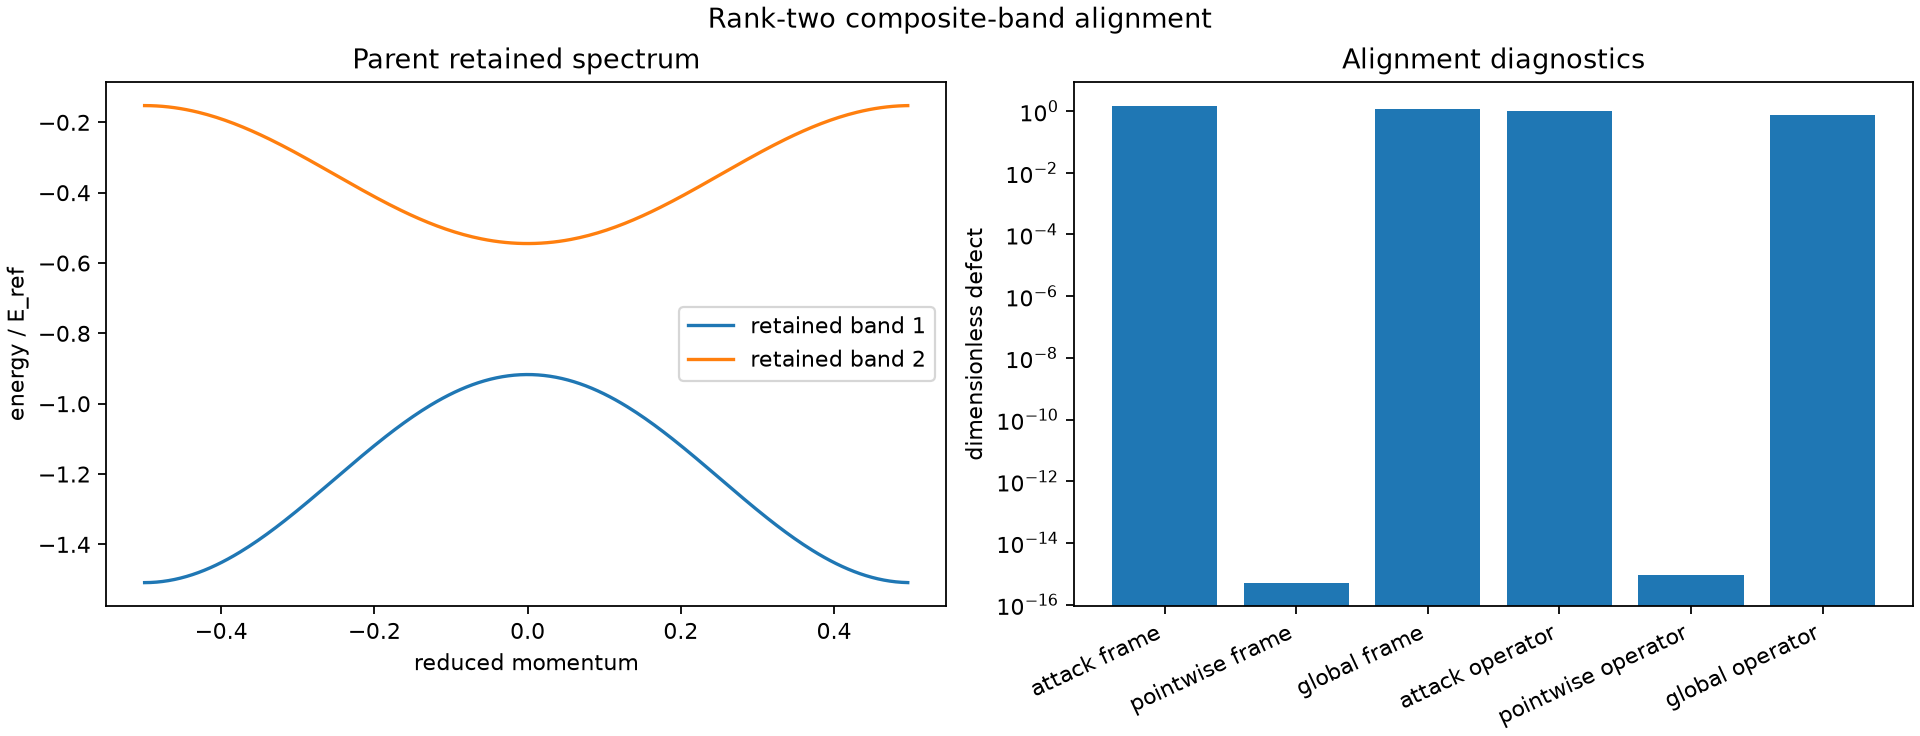
\includegraphics[width=\textwidth]{rank2-composite-alignment.png}
\caption{Authenticated finite alignment projection.  The left panel shows the two
retained parent eigenvalues on the disjoint evaluation mesh.  The right panel separates
attack, pointwise, and one-global-unitary frame and represented-operator defects.  The
logarithmic scale does not merge their mathematical meanings.}
\label{fig:alignment}
\end{figure}

The complete range inventory is reported in Table~\ref{tab:range-study}.  Reference and
pointwise results agree to roundoff throughout.  Their total evaluation errors decrease from
approximately $2.98\times10^{-1}\eref$ at onsite range to
$1.17\times10^{-14}\eref$ at range eight.  The attacked error decreases much more
slowly and remains $7.041355133552418\times10^{-5}\eref$ at range eight, approximately
$6.2\times10^{9}$ times the reference value there.  This ratio is a finite sampled
comparison, not an asymptotic decay rate.

\begin{table}[!htbp]
\centering
\caption{Complete finite range study.  Ordinary omitted norms $d$, construction total
errors $e_{\mathrm{con}}$, and disjoint-evaluation total errors $e_{\mathrm{eval}}$ are
in units of $\eref$.  R, A, and P denote reference, attacked, and pointwise channels.}
\label{tab:range-study}
\resizebox{\textwidth}{!}{%
\begin{tabular}{r@{\quad}rrr@{\quad}rrr@{\quad}rrr}
\toprule
& \multicolumn{3}{c}{Ordinary omitted block $L^2$ norm}
& \multicolumn{3}{c}{Construction total spectral maximum}
& \multicolumn{3}{c}{Evaluation total spectral maximum}\\
$R$ & $d_{\mathrm R}$ & $d_{\mathrm A}$ & $d_{\mathrm P}$
& $e_{\mathrm{R,con}}$ & $e_{\mathrm{A,con}}$ & $e_{\mathrm{P,con}}$
& $e_{\mathrm{R,eval}}$ & $e_{\mathrm{A,eval}}$ & $e_{\mathrm{P,eval}}$\\
\midrule
0 & $2.5450\mathrm e{-1}$ & $5.2350\mathrm e{-1}$ & $2.5450\mathrm e{-1}$ & $2.9789\mathrm e{-1}$ & $4.4454\mathrm e{-1}$ & $2.9789\mathrm e{-1}$ & $2.9789\mathrm e{-1}$ & $4.4454\mathrm e{-1}$ & $2.9789\mathrm e{-1}$\\
1 & $1.9754\mathrm e{-5}$ & $1.8512\mathrm e{-1}$ & $1.9754\mathrm e{-5}$ & $2.7573\mathrm e{-5}$ & $1.4768\mathrm e{-1}$ & $2.7573\mathrm e{-5}$ & $2.7565\mathrm e{-5}$ & $1.4898\mathrm e{-1}$ & $2.7565\mathrm e{-5}$\\
2 & $8.7006\mathrm e{-7}$ & $9.7439\mathrm e{-2}$ & $8.7006\mathrm e{-7}$ & $1.2269\mathrm e{-6}$ & $9.7312\mathrm e{-2}$ & $1.2269\mathrm e{-6}$ & $1.2261\mathrm e{-6}$ & $9.7379\mathrm e{-2}$ & $1.2261\mathrm e{-6}$\\
3 & $3.8719\mathrm e{-8}$ & $3.9152\mathrm e{-2}$ & $3.8719\mathrm e{-8}$ & $5.5322\mathrm e{-8}$ & $4.1515\mathrm e{-2}$ & $5.5322\mathrm e{-8}$ & $5.5259\mathrm e{-8}$ & $4.1531\mathrm e{-2}$ & $5.5259\mathrm e{-8}$\\
4 & $1.7453\mathrm e{-9}$ & $8.2797\mathrm e{-3}$ & $1.7453\mathrm e{-9}$ & $2.4856\mathrm e{-9}$ & $6.3755\mathrm e{-3}$ & $2.4856\mathrm e{-9}$ & $2.4869\mathrm e{-9}$ & $6.4296\mathrm e{-3}$ & $2.4869\mathrm e{-9}$\\
6 & $3.8610\mathrm e{-12}$ & $5.2560\mathrm e{-4}$ & $3.8609\mathrm e{-12}$ & $5.0475\mathrm e{-12}$ & $5.5446\mathrm e{-4}$ & $5.0472\mathrm e{-12}$ & $5.0389\mathrm e{-12}$ & $5.5899\mathrm e{-4}$ & $5.0389\mathrm e{-12}$\\
8 & $1.6352\mathrm e{-14}$ & $5.6539\mathrm e{-5}$ & $1.6370\mathrm e{-14}$ & $1.1435\mathrm e{-14}$ & $6.9238\mathrm e{-5}$ & $1.1324\mathrm e{-14}$ & $1.1657\mathrm e{-14}$ & $7.0414\mathrm e{-5}$ & $1.1546\mathrm e{-14}$\\
\bottomrule
\end{tabular}%
}
\end{table}

Figure~\ref{fig:locality} shows both the spectral consequence and the underlying
complete-block decay.  The reference and pointwise curves are visually coincident
because pointwise alignment recovers the reference represented operator.  The attacked
channel redistributes matrix weight over substantially more representatives.  Exact
pointwise band equivalence is therefore compatible with very different finite-range
locality.

\begin{figure}[!htbp]
\centering
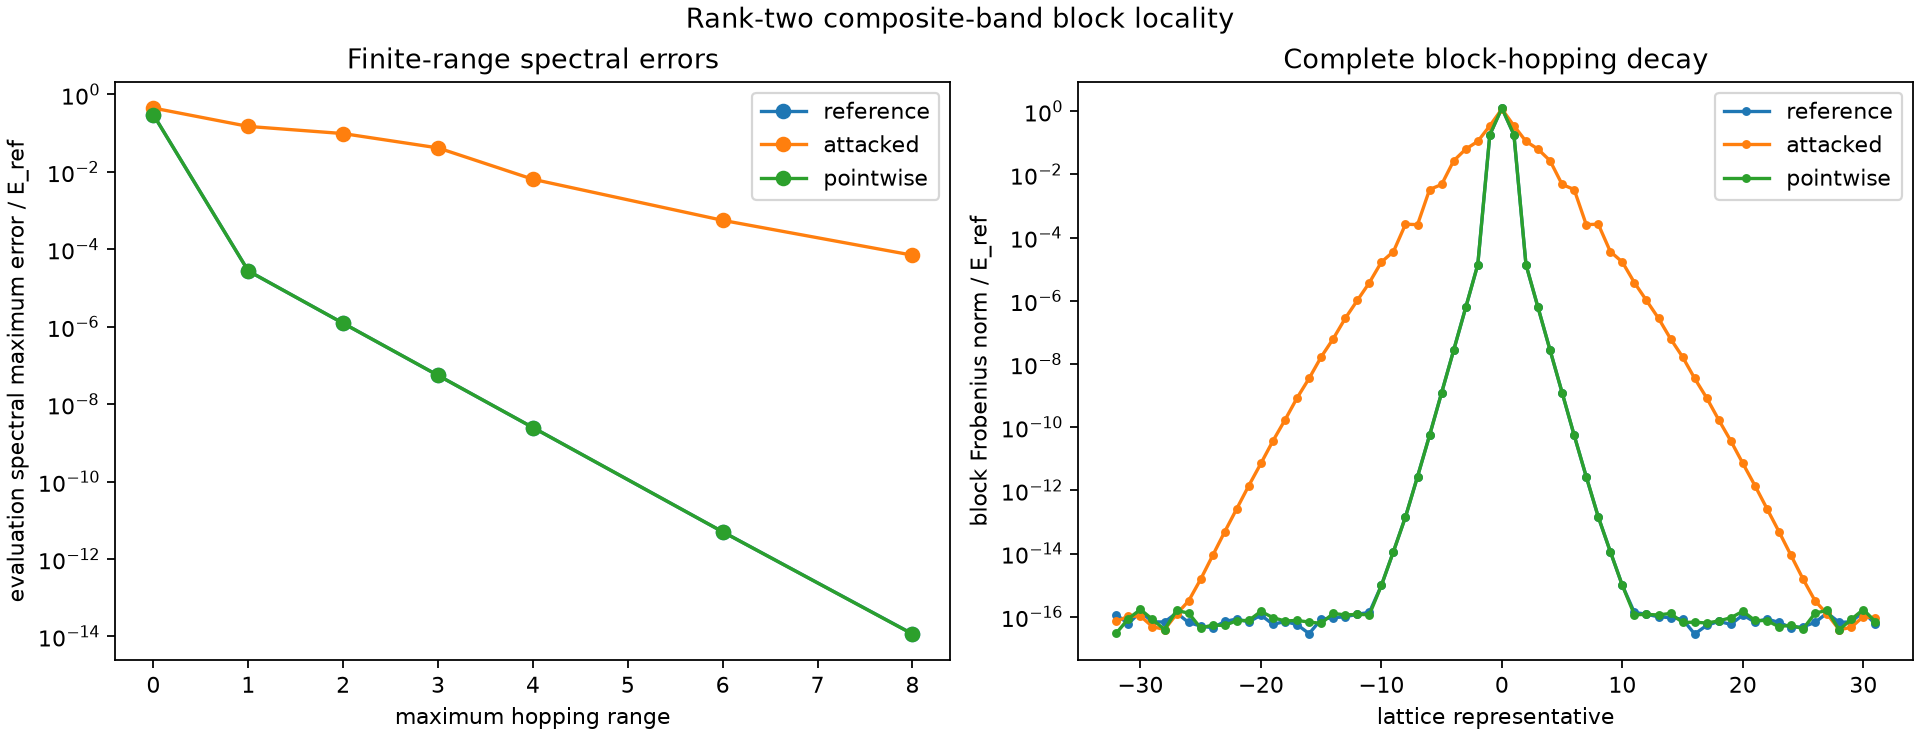
\includegraphics[width=\textwidth]{rank2-composite-locality.png}
\caption{Authenticated finite block-locality projection.  The left panel shows maximum
total ordered spectral error on the disjoint evaluation inventory for all seven ranges.  The
right panel shows the Frobenius norms of all 64 complete hopping blocks.  Coincidence of
reference and pointwise curves records recovery; the attacked tail records the declared
frame dependence.}
\label{fig:locality}
\end{figure}

\subsection{Separated error-channel accounting}

The complete ordinary reference interpolant is its own direct target, so its
interpolation residual is exactly zero under the implemented field definition.  For the
attacked channel, the maximum interpolation residual is
$1.524695274864153\times10^{-15}$ in normalized Frobenius error and
$1.998401444325282\times10^{-15}$ in sorted-band error.  The pointwise values are
$1.104000291768802\times10^{-15}$ and
$1.554312234475219\times10^{-15}$, respectively.  Thus finite interpolation remains at
binary64 scale and does not explain the displayed attacked range trend.

At range four, the attacked deliberate-truncation and total normalized errors are
\begin{align}
 \delta_{H,\mathrm{trunc}} &= 9.142140906351088\times10^{-3}, &
 \delta_{H,\mathrm{total}} &= 9.142140906351100\times10^{-3},\\
 \delta_{E,\mathrm{trunc}} &= 6.429588433655875\times10^{-3}, &
 \delta_{E,\mathrm{total}} &= 6.429588433655653\times10^{-3}.
\end{align}
At range eight, the attacked truncation and total sorted-band errors are
$7.041355133541316\times10^{-5}$ and $7.041355133552418\times10^{-5}$,
respectively.  Their near equality is an
observed consequence of the roundoff-scale interpolation channel, not an assumption
that maxima add.

\begin{figure}[!htbp]
\centering
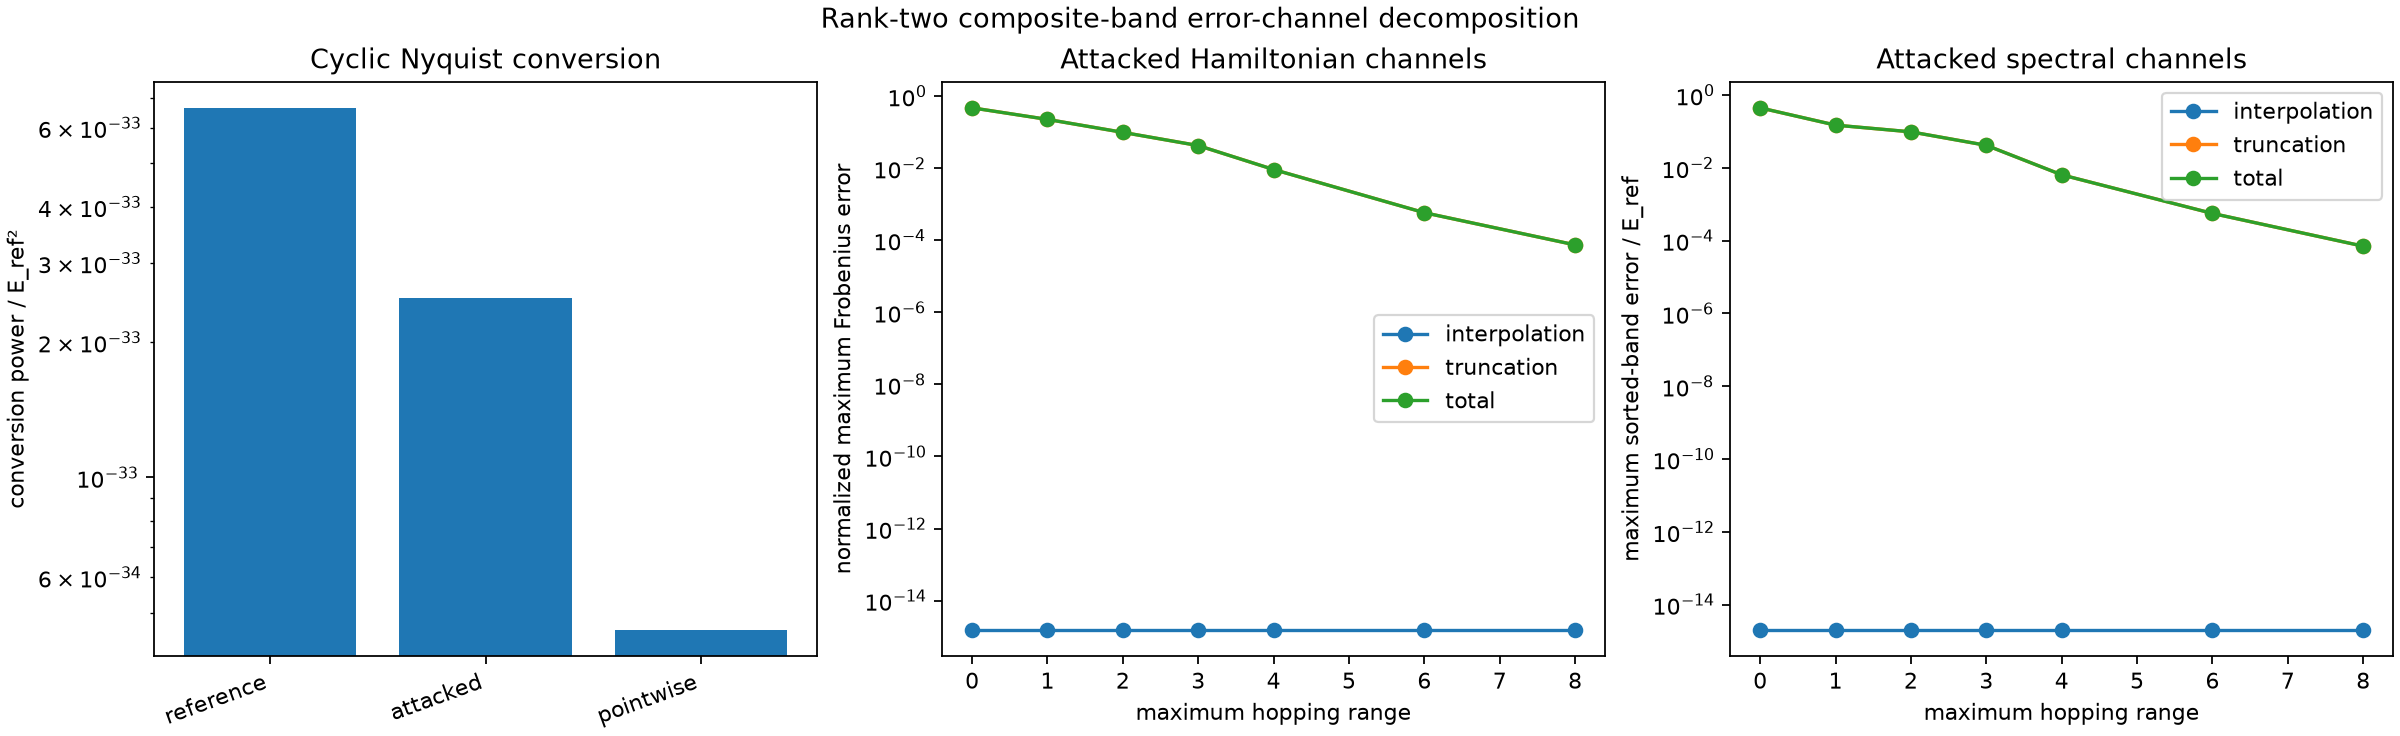
\includegraphics[width=\textwidth]{rank2-composite-error-channels.png}
\caption{Authenticated error-channel decomposition.  The left panel reports normalized
negative-Nyquist conversion power separately from off-node errors.  The center and
right panels show the attacked channel's interpolation, deliberate-truncation, and total
maximum residuals in normalized Hamiltonian and sorted-band metrics.  Lines connect the
seven declared ranges as guides to the eye; the channels are not stacked or summed.}
\label{fig:error-channels}
\end{figure}

No application-error threshold or preferred hopping range is declared by this protocol.
Consequently the calculation supports a comparison of channels, not a range-selection
or admissibility claim.

\FloatBarrier
\section{Independent verification and authenticated presentation}

The producer uses PhysKit dense complex-Hermitian eigensystems, the
\code{ksdft2effmass} (KSD) polar frame-transport and represented-operator owners, and
the Project Koios Optimization batched
complex-unitary Procrustes solver.  The independent verifier does not call the producer
or that Procrustes solver.  It reconstructs the exact parent, canonical eigensystem
phases, frame transport, attacks, singular-value right actions, represented operators,
complete cyclic and ordinary Fourier sums, negative-Nyquist conversion power, direct
evaluation targets, block truncations, separated Hamiltonian and ordered-spectrum error
channels, diagnostics, and every field of the visualization projection using direct
NumPy and SciPy formulas.

The verifier independently applies Equation~\eqref{eq:rank-cutoff} and rejects any
pointwise or global covariance at or below the selected cutoff.  Shared binary64, Basic Linear Algebra Subprograms (BLAS), Linear Algebra PACKage
(LAPACK), NumPy, and SciPy lineage remains a disclosed limitation; this is an
independent software route rather than an independent physical experiment.

All 56 named comparisons passed.  The maximum observed discrepancy was
$1.4210854715202004\times10^{-14}$, below the applicable stored tolerances.  The result,
verification aggregate, and visualization projection each survive canonical byte-identical JavaScript Object Notation (JSON)
round trips.  Rendering admits exact stored bytes only after
recomputing and exact-comparing both verification and projection values.

The three Portable Network Graphics (PNG) files embedded in
Figures~\ref{fig:alignment}, \ref{fig:locality}, and~\ref{fig:error-channels} were
produced from the authenticated projection at 160 dots per inch.  They contain no newly
calculated scientific value and are report-local review illustrations rather than
retained execution artifacts.

\section{Historical parity and convention boundary}

The direct source is the bounded scientific successor to the historical M2 calculation,
but it does not decode or wrap historical campaign schemas.  Named finite channels
reproduce historical M2 values within the direct $10^{-11}$ energy tolerance, including
the sampled gap, overlap conditioning, frame and operator defects, omitted-block norms,
and construction spectral errors.  For example, the historical and direct attacked
construction errors at range four are respectively
$0.006375530149533293\eref$ and $0.006375530149533404\eref$.

The direct lifecycle uses current canonical KSD transport and centered Fourier owners.
It therefore does not assert byte-identical closure phases, hopping blocks, or every
attacked evaluation value.  At range four, historical M2 reports an attacked evaluation
error of $0.006429434409208734\eref$, while the direct source reports
$0.006429588433655653\eref$.  This explicit adaptation prevents a compatibility
transformation from hiding the current convention.  Historical publication claims
remain bound to their original result and verification bytes.

\section{Provisional provenance}

The in-memory development calculation used branch
\nolinkurl{work/periodic1d-composite-alignment-v3} at base revision
\nolinkurl{8cf9e93d7c3d791f81ee119476328970fe5632ba} in a dirty worktree.  The local
software environment reported Python 3.14.6, ksdft2effmass 0.1.0.dev0,
projectkoios-physkit 0.1.3.dev0, projectkoios-optimization 0.1.0.dev0, NumPy 2.5.1,
SciPy 1.18.0, and Matplotlib 3.11.1.  These versions describe the review environment;
they do not create a retained execution contract.

Exact 256-bit Secure Hash Algorithm (SHA-256) identities for the provisional review
bytes are:
\begin{itemize}
 \item configuration bytes: \nolinkurl{08ad9c6d967616e5b286ece1a3296b2ed65bdce672daacaecf26b933e04ca4b6};
 \item result bytes: \nolinkurl{7c8a65f14f480c22e4eeeeae26f56ef7f0116accec0a16f80bb7c0cf7931f0f7};
 \item verification bytes: \nolinkurl{72d65f4c67ec0a76b23b333317afbc16736980e877ba0f6f0dffcbf0e56d5102};
 \item visualization-data bytes: \nolinkurl{578d8270188d25087091862bdb276ff818975f18df051b5a9615ff6f6a5fb1fa};
 \item alignment report PNG: \nolinkurl{56efc40bf7a2772aa8bcd1736531fe74c24282c7f187229606edb05864c46107};
 \item locality report PNG: \nolinkurl{52292ea400ea10cc5efe6bf2845c3e52b50e47b423cc22b99a6743392813d9ee};
 \item error-channel report PNG: \nolinkurl{0616267e2999429310667a52c91cdfc5badc399154ea98f1e0ee502220c2f10d}.
\end{itemize}
The canonical result, verification, and visualization documents contained 961263,
25618, and 45390 bytes respectively.  SHA-256 establishes byte identity only; it does
not establish scientific validity, authorship, rights, publication, release, or
sealing.  No retained successor result or verification file exists in the repository.

\section{Discussion}

\subsection{What is invariant and what is representation-dependent}

The retained projector and complete pointwise spectrum are invariant under the declared
right-unitary attack.  The represented matrix field, its block coefficients, and the
spectra of its finite-support truncations are not.  This distinction is the main
scientific result.  It prevents a band-only comparison from being interpreted as a
complete statement about representation efficiency.

The pointwise oracle is especially important.  Its recovery of the reference channel at
roundoff confirms that the longer attacked tail is not caused by changing the retained
subspace or losing spectral information.  The global residual shows a different fact:
one restricted constant action cannot reproduce a momentum-dependent inverse.  These two
alignment families must not be merged into one generic ``alignment error.''

\subsection{Why complete-transform closure precedes locality claims}

All three complete transforms reconstruct their construction matrix fields at
roundoff.  The range study therefore compares deliberate finite-support projections of
closed finite transforms.  Without this benchmark, a large attacked range error could
be caused by transform normalization, representative ordering, cyclic Hermiticity, or
incomplete reconstruction.  The ordered protocol excludes those alternatives before
interpreting locality.

The disjoint evaluation mesh provides an additional safeguard.  Construction errors
measure the finite transform on the data used to build it; evaluation errors probe newly
sampled fields.  Direct evaluation targets separate complete-interpolant discrepancy
from deliberate support deletion and their total consequence.  The removed cyclic
Nyquist block remains a fourth, power-valued convention channel rather than an off-node
spectral error.  Interpolation remains at roundoff while the attacked truncation channel
follows the displayed range trend.  This supports the finite truncation interpretation;
it does not prove a continuum error bound.

\subsection{Relation to the scalar control}

The rank-one controlled-four-state report establishes that spectral reduction alone can
produce a scalar Fourier tail even though scalar $U(1)$ conjugation is exactly inert.
The present rank-two control adds the missing internal action: a nonconstant $U(2)$
right rotation redistributes the represented matrix field by the block convolution in
Equation~\eqref{eq:block-convolution}.  The scalar and rank-two reports therefore form a
mechanism-separation pair:
\begin{itemize}
 \item rank one isolates spectral reduction, interpolation, and truncation without
       gauge-dependent represented-operator locality;
 \item rank two holds the retained subspace and complete spectrum fixed while activating
       momentum-dependent internal frame structure.
\end{itemize}
This comparison is methodological support for the scientific lineage of Ragasa2026a.
The repository's current allocation ledger assigns the direct composite-alignment family
to Ragasa2026c rather than the active Ragasa2026a evidence graph.  Changing that
publication allocation or binding these bytes into a manuscript manifest is a separate
reviewed action; the technical report does not silently perform it.

\subsection{Historical M2 and current canonical conventions}

The named M2 parity values show continuity with the historical finite control while the
range-four evaluation difference exposes a real convention boundary.  Treating the
historical and direct bytes as identical would require a compatibility transformation
that obscures the current owners.  The report instead preserves both values and explains
why the direct source uses its own canonical transport and centered transform.

\section{Limitations and nonclaims}

The finite control does not establish:
\begin{itemize}
 \item a continuum limit or a globally certified retained/excluded gap;
 \item uncertainty quantification or a forward-error bound for every reported digit;
 \item robustness under changes of parent coefficients, construction size, evaluation
       inventory, attack family, support rule, or tolerance;
 \item a universal exponential-localization law or universal hopping-range inflation;
 \item material applicability, density-functional-theory accuracy, or successful
       Wannierization;
 \item a topological interpretation of the closure eigenphases;
 \item higher-rank real or complex gauge behavior;
 \item an application threshold or a selected scientifically adequate range;
 \item publication acceptance, retained evidence, release, sealing, or a Project
       Koios--Formal certificate.
\end{itemize}
The one-global-unitary residual is diagnostic of the declared restricted family only.
It is not a distance between physical systems.  The attacked and reference complete
fields remain pointwise unitarily equivalent.

The M3 admissible-set consumers now admit authenticated canonical composite-result
bytes and explicit verification dependencies.  After that migration passed review, the
live M2 runtime was retired without a compatibility facade.  Its final source bytes and
historical calculation artifacts remain recoverable provenance; they are not successor
runtime inputs.

\section{Conclusions}

Within the 64-point construction and exactly disjoint 257-point evaluation control, the
retained rank-two parent space is sampled-separated and the polar transport overlaps are
well conditioned.  The prescribed momentum-dependent right action preserves the
retained projector and complete pointwise spectra while substantially changing the
represented matrix field.  Pointwise Procrustes alignment recovers the reference frame,
projector, known inverse, and represented operator at roundoff.  A single global unitary
cannot recover the nonconstant attack.

The complete cyclic transforms close at roundoff, their negative-Nyquist conversion
powers are separately negligible, and the complete ordinary interpolants agree with
their direct targets at roundoff.  The reported attacked range trend is therefore in the
deliberate-truncation channel rather than transform failure, convention conversion, or
finite interpolation.  Reference
and pointwise-aligned blocks decay rapidly and reach roundoff-scale range-eight errors.
The attacked blocks have a much longer tail and retain an evaluation error near
$7.04\times10^{-5}\eref$ at range eight.  Exact pointwise band equivalence therefore
does not determine finite block-hopping locality without a declared frame and support
convention.

The full technical record contains the analytic mechanism, seven benchmarks, complete
finite range inventory, independent reconstruction, historical parity boundary,
literature position, provenance, and explicit nonclaims.  That is the upstream level
from which publication prose should be distilled.  Retention or promotion still
requires independent review, separately authorized direct execution, and the repository
provenance and sealing gates.

\appendix

\section{Frozen control inventory}

\begin{table}[htbp]
\centering
\caption{Declared controls for the provisional rank-two calculation.}
\small
\begin{tabular}{ll}
\toprule
Control & Value \\
\midrule
Parent / retained dimensions & $4/2$ \\
Construction / evaluation sizes & $64/257$ \\
Evaluation shift & $1/65$ of one evaluation step \\
Ranges & $0,1,2,3,4,6,8$ \\
Attack angle & $0.30+0.65\sin(2\pi k)+0.30\sin(4\pi k)$ \\
Gap threshold & $0.5\eref$ \\
Overlap singular-value threshold & $0.8$ \\
Absolute / relative rank controls & $10^{-14}/10^{-12}$ \\
Energy / dimensionless tolerances & $10^{-11}\eref/10^{-12}$ \\
Cyclic / ordinary representatives & $-32,\ldots,31$ / $-31,\ldots,31$ \\
Error channels & conversion power; interpolation, truncation, total \\
Locality channels & reference, attacked, pointwise \\
Diagnostic-only alignment & one global unitary \\
\bottomrule
\end{tabular}
\end{table}

\section{Interpretation map}

\begin{center}
\begin{tabular}{L{0.24\textwidth}L{0.31\textwidth}L{0.35\textwidth}}
\toprule
Object & What it establishes & What it does not establish \\
\midrule
Sampled gap & Finite retained/excluded separation & Global isolation certificate \\
Overlap singular value & Finite transport conditioning & Canonical backend-independent frame \\
Projector defect & Retained-space agreement & Represented-matrix agreement \\
Pointwise oracle & Known inverse recovery & Restricted global recovery \\
Global Procrustes residual & Best declared constant action & Physical inequivalence \\
Complete transform closure & Finite transform correctness & Locality or adequacy \\
Conversion power & Removed cyclic Nyquist weight & Off-node spectral error \\
Interpolation error & Complete interpolant versus direct field & Deliberate support loss \\
Truncation error & Finite range versus complete ordinary field & Total consequence \\
Total error & Finite range versus direct field & Sum of independent scalar errors \\
Omitted block norm & Ordinary coefficient-tail norm & Universal spectral-error law \\
SHA-256 digest & Exact byte identity & Scientific validity or sealing \\
\bottomrule
\end{tabular}
\end{center}

\footnotesize
\bibliographystyle{plain}
\bibliography{references}

\end{document}
